\chapter{Implementacja} \label{chap:implementacja}
Rozdział ten skupia się na implementacji projektu, którym jest rekonstrukcja aplikacji internetowej stworzonej przy pomocy Reacta i Reduxa, w formie aplikacji napisanej w języku Elm. Opisane są w~nim założenia przyjęte w trakcie tworzenia aplikacji, uzyskany efekt oraz problemy napotkane w czasie implementacji.

\section{Założenia i uzyskany efekt}
Aplikacją, która została wybrana do rekonstrukcji w języku Elm, jest projekt stworzony przez grupę studentów uczelni Akademii Górniczo-Hutniczej. Aplikacja Zmora jest zautomatyzowaną platformą edukacyjną, skierowaną głównie do studentów kierunków informatycznych \cite{zmoraUi}. Jednym z jej elementów jest interfejs aplikacji internetowej stworzony głównie przy pomocy kombinacji Reacta i Reduxa.

Ze względu na rozbudowaną strukturę i ilość widoków dostępnych w aplikacji zostały wybrane tylko dwa. Jednym z nich jest strona główna aplikacji przedstawiona na rysunku \ref{fig:homOrg}, która poza górnym panelem oraz menu położonym z lewej strony, jest statyczną stroną, niepobierającą żadnych danych z~zewnątrz. Aby uwzględnić także komunikację z serwerem aplikacji, drugim wybranym widokiem jest strona logowania widoczna na rysunku \ref{fig:logOrg}. Czerwona linia oznacza te elementy widoku, które zostały uwzględnione przy rekonstrukcji. Znajdujący się po prawej stronie fragment odpowiedzialny za rejestrację nowych użytkowników nie został uwzględniony aby nie dodawać niepotrzebnych użytkowników.

\begin{figure}[h]
	\centering
	\begin{subfigure}{0.5\textwidth}
		\centering
		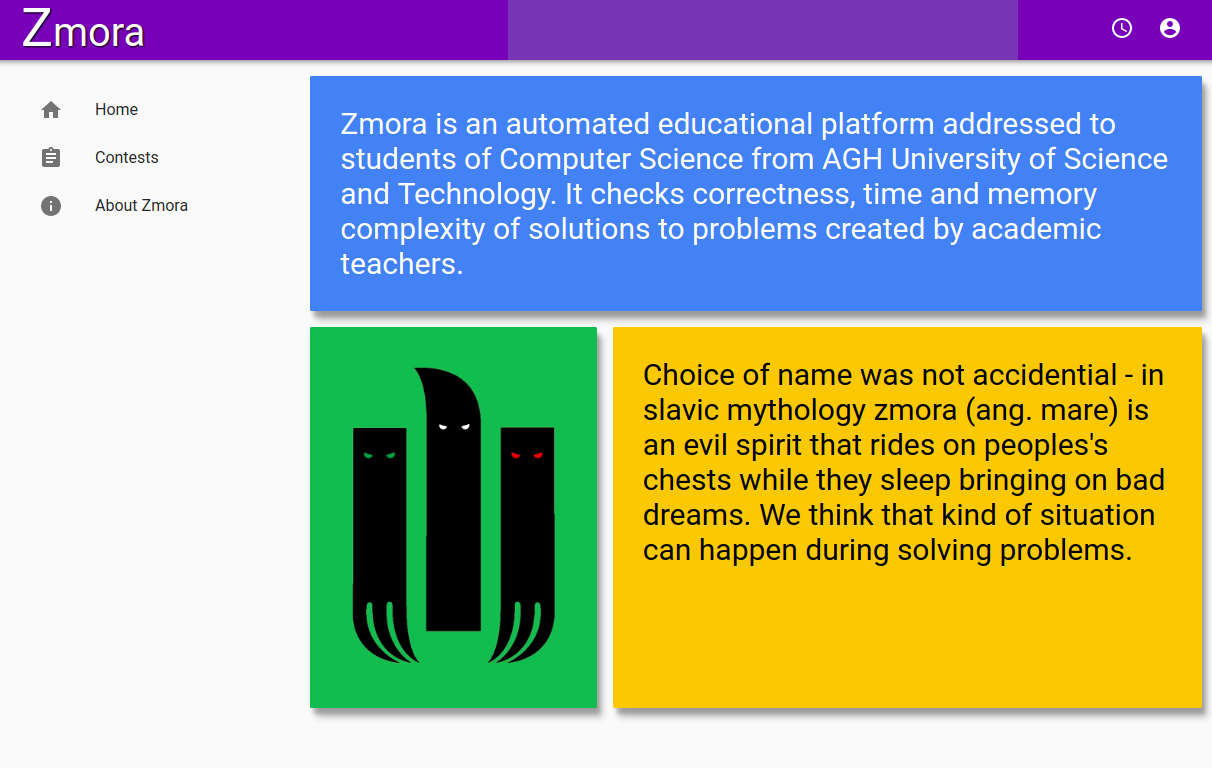
\includegraphics[width=0.9\linewidth]{images/homepage_zmora}
		\caption{Oryginalny widok strony głównej}
		\label{fig:homOrg}
	\end{subfigure}%
	\begin{subfigure}{0.5\textwidth}
		\centering
		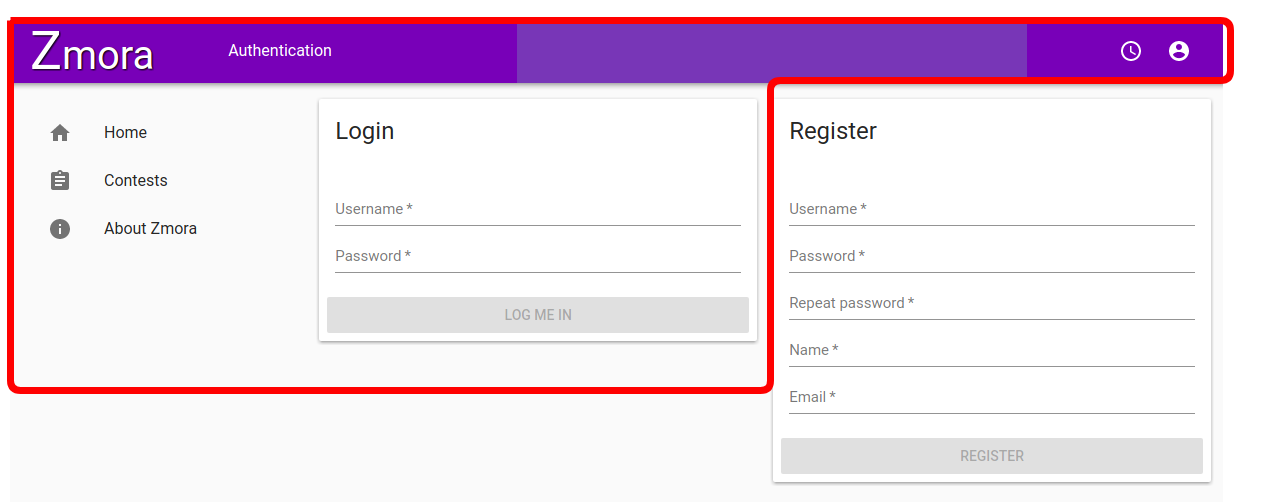
\includegraphics[width=0.9\linewidth]{images/login_zmora}
		\caption{Oryginalny widok strony logowania}
		\label{fig:logOrg}
	\end{subfigure}
	\label{fig:orgView}
	\caption{Widoki wybrane do zrekonstruowania}
\end{figure}

Ze względu na przyjęte w założeniach ograniczenia co do widoków, końcowy efekt mimo podobnego wyglądu w stosunku do oryginału różni się pod kilkoma względami. Menu boczne aplikacji znajdujące się na obu podstronach zgodnie z założeniami oryginalnej wersji aplikacji przenosi pod dokładnie te same adresy, jednak z powodu braku zaimplementowanych widoków zostaje wyświetlony dodatkowy widok stworzony specjalnie dla nie znalezionych stron. Porównując widok strony głównej w wersji oryginalnej oraz zrekonstruowanej przy pomocy języka Elm, ciężko dostrzec między nimi różnice. W~przypadku widoku strony logowania można zauważyć drobne przesunięcia obiektów w stosunku do oryginału. Wynikało to przede wszystkim z różnicy używanych bibliotek. W trakcie tworzenia rekonstrukcji jedynymi bibliotekami odpowiadającymi za widok były pakiety udostępnione przez menedżer pakietów elm-package, oraz style w postaci plików CSS.
\begin{figure}[h]
	\begin{subfigure}{0.5\textwidth}
		\centering
		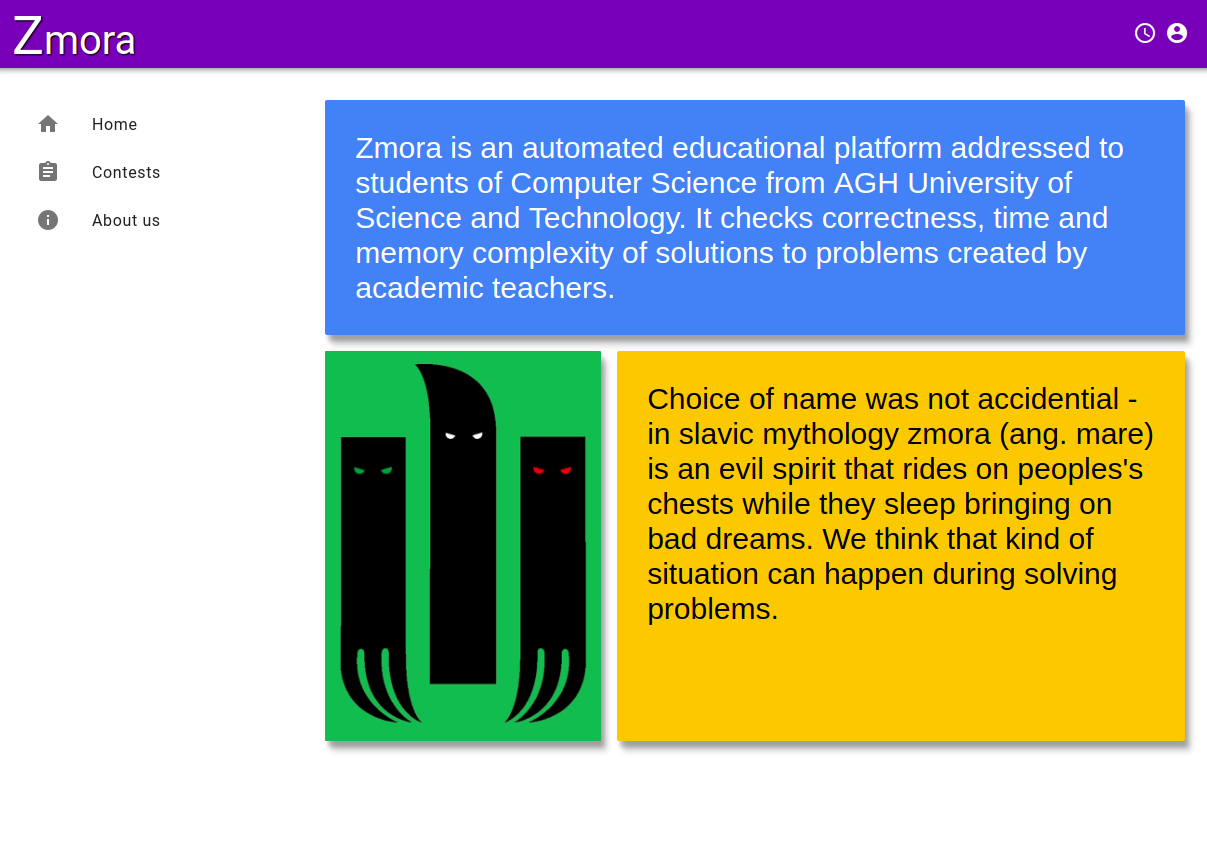
\includegraphics[width=0.9\linewidth]{images/homepage_elm}
		\caption{Zrekonstruowany widok strony logowania}
		\label{fig:homElm}
	\end{subfigure}%
	\begin{subfigure}{0.5\textwidth}
		\centering
		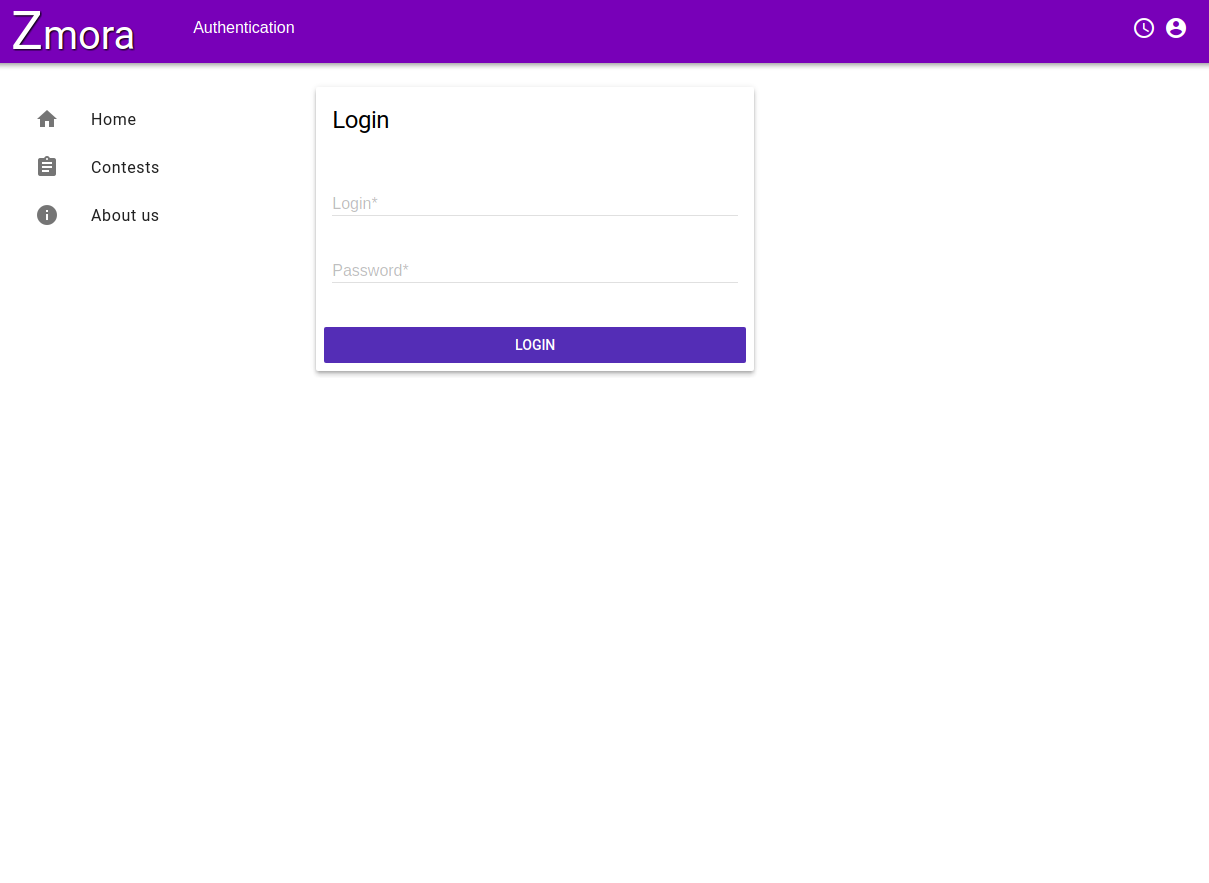
\includegraphics[width=0.9\linewidth]{images/login_elm}
		\caption{Zrekonstruowany widok strony logowania}
		\label{fig:logElm}
	\end{subfigure}
	\caption{Zrekonstruowane widoki stworzone przy pomocy języka Elm}
	\label{fig:elmView}
\end{figure}

\section{Napotkane problemy}
Głównym problemem, jaki został napotkany podczas rekonstrukcji aplikacji była dostępność bibliotek służących do budowania widoku oraz obsługi danych. Widok aplikacji w przypadku oryginału był budowany za pomocą komponentów biblioteki Material-UI, która implementuje styl Material Design. Jest to styl graficzny stworzony przez firmę Google, którego założeniem była prostota, czytelność i~łatwość dostosowania do różnych płaszczyzn. Niestety, menedżer pakietów, z którego korzystał Elm, oferował jedynie bibliotekę będącą portem uboższej wersji Material Designa o nazwie Material Design Lite. Spowodowało to, że proste komponenty, takie jak górna belka aplikacji, które w oryginalnej implementacji zajmowały kilka linijek kodu, w zrekonstruowanej wersji stawały się ogromnymi elementami, które trzeba było modyfikować za pomocą własnych stylów.

Dużym problemem było także znalezienie biblioteki do obsługi danych. Serwer aplikacji oferuje zarządzanie danymi poprzez zapytania języka GraphQL. W przypadku oryginalnej implementacji została użyta biblioteka stworzona przez twórców API, z którego korzystał serwer. Będąc pakietem specjalnie skonstruowanym dla Reacta, umożliwiała szybkie i proste definiowanie zapytań przy pomocy składni języka GraphQL. Aby skorzystać z podobnej funkcjonalności w zrekonstruowanej wersji aplikacji, wykorzystano oferowaną w menedżerze pakietów npm bibliotekę, która na podstawie plików zawierających treść zapytań w języku GraphQL oraz konfiguracji typów pobieranej z serwera, generowała pliki z~kodem Elma, zawierające funkcje oraz typy umożliwiające korzystanie z zapytań do serwera wewnątrz kodu aplikacji. Niestety API wystawione przez serwer nie było w pełni uwzględnione w konfiguracji serwera. Dane, które były zwracane przez serwer, były opakowywane w dodatkowy obiekt, co powodowało, że przy próbie dekodowania danych do typów języka Elm operacja kończyła się niepowodzeniem. Jedynym możliwym rozwiązaniem okazało się zmodyfikowanie biblioteki generującej moduły Elma w~taki sposób, aby niezależnie od podanego zapytania ostateczne dane były opakowywane w dodatkowy typ.

Inną trudnością, która wystąpiła podczas rekonstrukcji oryginalnych widoków, było zaprojektowanie modelu danych. W przeciwieństwie do kombinacji Reacta i Reduxa, które bazując na JavaScript'cie nie są ograniczone przez typy i mogą modyfikować w każdej chwili stan, dodając do niego kolejne pola. W~przypadku Elma model danych jest ustalony z góry przez silne typowanie, przez co model musiał być zaprojektowany tak, aby uwzględnić każdy przypadek danych otrzymywanych od serwera. Dodatkowym utrudnieniem było trzymanie opcji dotyczących widoku razem z danymi aplikacji. To wszystko powodowało, że stan aplikacji stawał się po jakimś czasie obiektem o skomplikowanej strukturze, który dodatkowo był ograniczony przez typy, co wymuszało przewidzenie wszystkich możliwych sytuacji zmiany stanu bez możliwości praktycznego przetestowania aplikacji.